% Source: Code/CommonSenseCarolina/latex/sg-election-turnout.tex
\documentclass[border=0pt]{standalone}
\usepackage{pgfplots}
\usepackage{xcolor}
\usepackage{tikz}

\pgfplotsset{compat=1.18}

\definecolor{Garnet}{HTML}{73000A}
\definecolor{GarnetDark}{HTML}{4A0006}
\definecolor{Atlantic}{HTML}{466A9F}
\definecolor{Congaree}{HTML}{1F414D}
\definecolor{Rose}{HTML}{CC2E40}
\definecolor{Horseshoe}{HTML}{65780B}
\definecolor{Black90}{HTML}{363636}
\definecolor{Black70}{HTML}{5C5C5C}
\definecolor{Black50}{HTML}{A2A2A2}
\definecolor{Black30}{HTML}{C7C7C7}
\definecolor{Black10}{HTML}{ECECEC}
\definecolor{GridDark}{HTML}{2A2A2A}
\definecolor{BgTop}{HTML}{000000}
\definecolor{BgBottom}{HTML}{000000}

\newcommand{\ballot}[4]{% x, y, scale, opacity
  \begin{scope}[shift={(#1,#2)}, scale=#3, opacity=#4]
    \draw[Garnet, line width=1.4pt] (0,0) rectangle (0.4,0.4);
    \draw[Garnet, line width=0.8pt] (0.08,0.18) -- (0.16,0.08) -- (0.34,0.32);
  \end{scope}
}

\begin{document}
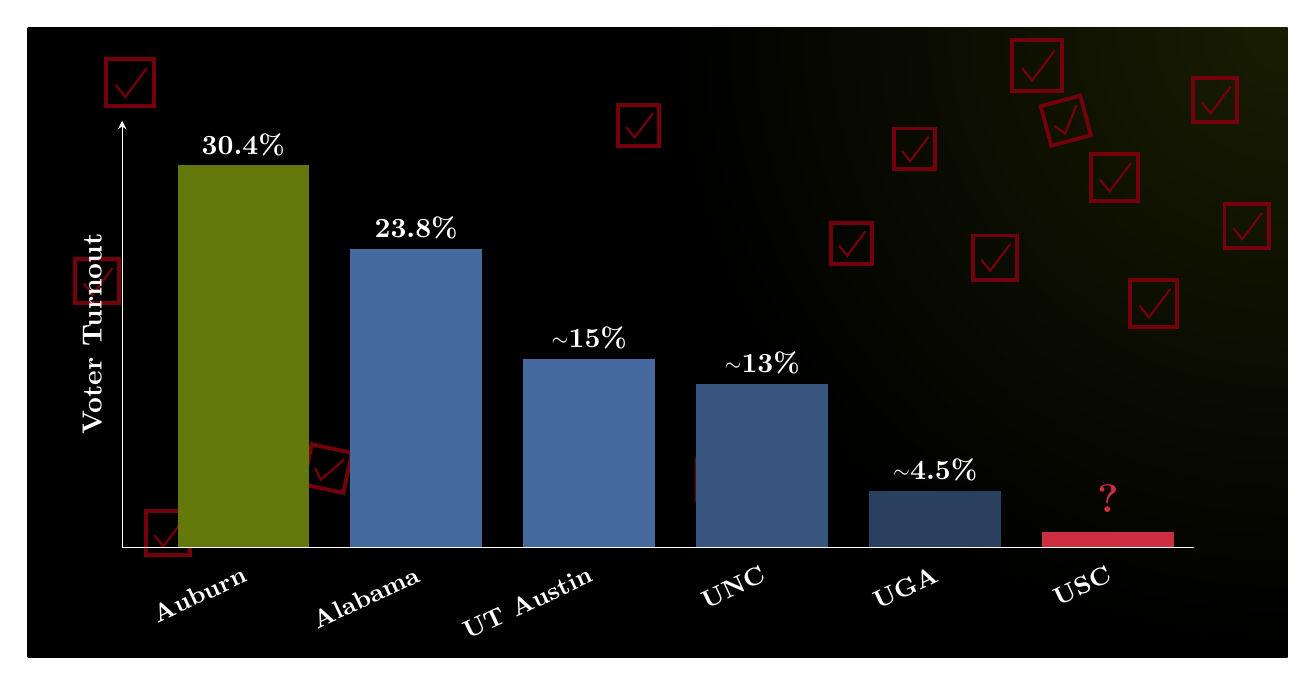
\begin{tikzpicture}

% 2:1 ratio background
\shade[top color=BgTop, bottom color=BgBottom] (0,0) rectangle (16,8);


% Subtle green glow from top right
\begin{scope}
  \clip (0,0) rectangle (16,8);
  \shade[inner color=Horseshoe, outer color=BgTop, opacity=0.25] (16,8) circle (8);
\end{scope}

% Scattered ballot checkboxes (behind chart) — spread across entire image
% Scattered ballot checkboxes — concentrated top-right, some elsewhere
% Top-right cluster
\ballot{12.5}{7.2}{1.6}{1.0}
\ballot{14.8}{6.8}{1.4}{1.0}
\ballot{11.0}{6.2}{1.3}{1.0}
\ballot{13.5}{5.8}{1.5}{1.0}
\ballot{15.2}{5.2}{1.4}{1.0}
\ballot{10.2}{5.0}{1.3}{1.0}
\ballot{14.0}{4.2}{1.5}{1.0}
\ballot{12.0}{4.8}{1.4}{1.0}
\begin{scope}[rotate around={15:(13.0,6.5)}]
  \ballot{13.0}{6.5}{1.3}{1.0}
\end{scope}
% Scattered elsewhere
\ballot{1.0}{7.0}{1.5}{1.0}
\ballot{7.5}{6.5}{1.3}{1.0}
\ballot{0.6}{4.5}{1.4}{1.0}
\ballot{5.0}{3.5}{1.5}{1.0}
\ballot{1.5}{1.3}{1.4}{1.0}
\ballot{8.5}{2.0}{1.3}{1.0}
\begin{scope}[rotate around={-12:(3.5,2.2)}]
  \ballot{3.5}{2.2}{1.3}{1.0}
\end{scope}

\begin{axis}[
    at={(1.2cm,1.4cm)},
    width=15.2cm,
    height=7cm,
    xmin=0.3, xmax=6.5,
    ymin=0, ymax=34,
    xtick={1,2,3,4,5,6},
    xticklabels={Auburn, Alabama, UT Austin, UNC, UGA, USC},
    xticklabel style={font=\small\bfseries, color=white, rotate=25, anchor=north east},
    x tick label style={yshift=-2pt},
    ytick=\empty,
    ylabel={Voter Turnout},
    ylabel style={font=\normalsize\bfseries, color=white, at={(axis description cs:-0.01,0.5)}},
    ymajorgrids=false,
    axis x line*=bottom,
    axis y line=left,
    y axis line style={color=white},
    x axis line style={color=white},
    tick style={draw=none},
    clip=false,
]

% Bar width in axis units
\def\bw{0.38}

% Auburn - 30.4%
\fill[Horseshoe] (axis cs:{1-\bw},0) rectangle (axis cs:{1+\bw},30.44);
\node[font=\normalsize\bfseries, color=white, anchor=south] at (axis cs:1,30.44) {30.4\%};

% Alabama - 23.8%
\fill[Atlantic] (axis cs:{2-\bw},0) rectangle (axis cs:{2+\bw},23.8);
\node[font=\normalsize\bfseries, color=white, anchor=south] at (axis cs:2,23.8) {23.8\%};

% UT Austin - ~15%
\fill[Atlantic] (axis cs:{3-\bw},0) rectangle (axis cs:{3+\bw},15);
\node[font=\normalsize\bfseries, color=white, anchor=south] at (axis cs:3,15) {{\raise.17ex\hbox{$\scriptstyle\sim$}}15\%};

% UNC - ~13%
\fill[Atlantic!80!black] (axis cs:{4-\bw},0) rectangle (axis cs:{4+\bw},13);
\node[font=\normalsize\bfseries, color=white, anchor=south] at (axis cs:4,13) {{\raise.17ex\hbox{$\scriptstyle\sim$}}13\%};

% UGA - ~4.5%
\fill[Atlantic!60!black] (axis cs:{5-\bw},0) rectangle (axis cs:{5+\bw},4.5);
\node[font=\normalsize\bfseries, color=white, anchor=south] at (axis cs:5,4.5) {{\raise.17ex\hbox{$\scriptstyle\sim$}}4.5\%};

% USC - ?
\fill[Rose] (axis cs:{6-\bw},0) rectangle (axis cs:{6+\bw},1.2);
\node[font=\Large\bfseries, color=Rose, anchor=south] at (axis cs:6,2) {?};

\end{axis}
\end{tikzpicture}
\end{document}
